\documentclass[a4paper]{article}

\usepackage{a4wide}
\usepackage[utf8]{inputenc}
\usepackage[T1]{fontenc}
\usepackage{graphicx}
\usepackage{float}

\bibliographystyle{alpha}

%Alternative paragraph style
\setlength{\parindent}{0.0in}
\setlength{\parskip}{0.1in}

%Adjust footnote size to larger than normal text size
\let\footnotesize\normalsize

\begin{document}

\large

\title{Explanation Architecture for Companion Systems}
\author{Tamino Hartmann}
\date{\today}

\maketitle

\begin{abstract}
\normalsize

In this paper, we take a look at how to strengthen the trust between a companion system and a user by utilizing explanations based on the original paper \cite{origin}. These explanations should be constructed to fit the issue of trust at stake while acknowledging the user's own knowledge so that a learning effect can be achieved. We also look at how we can bring the system to give explanations without that the user asked for one in a dialogue, when appropriate. A proposed architecture for a companion system capable of utilizing such explanations is also presented.
\end{abstract}
\newpage

\section{Introduction}

When users buy a new electronic device such as a smartphone, they often look at the advertised features listed on the box. Most pick out the few features that are important to themselves while others simply compare the length of the list. However even if a user buys a new smartphone for a new feature, the purchase does not come with an instant understanding of the feature. Once unpacked at home, the user is then faced with finding the feature and learning to use it – a task that is often not without its problems. If the hurdle is deemed too large, the new gadget is perceived to be a disappointment. Said frankly, you could say that the user is unwilling to cooperate with the device.

Changing this is the main purpose of the paper "Explanation Architecture for Companion Systems" \cite{origin}. It expands on the idea of providing an explanation architecture, primarily for systems that offer a user dialogue. The aim of providing explanations is to strengthen a user's willingness to work with the system to solve problems or complete tasks. Apart from simply explaining new things to a user, such a system can also be used to cooperate with a user on tasks such as creating the user's calendar with given constraints such as time restrictions and travel times.

\paragraph{Companion Systems.} The original paper concentrates on so-called {\it companion systems}. Companion systems are systems that assist a user in a multitude of day-to-day tasks, such as the aforementioned scheduling of appointments. However, the capabilities of a companion system do not stop there. Using a vast array of knowledge, these systems can also help a user with a new and unknown task, tasks that are out of a user's comfort zone. To make the most of such a system, this architecture is deployed using a range of modules, so as to make it easy to include any available device to help the user. However, the core system should be based upon a device that the user keeps with her the entire day. This could, for example, be a smartphone. An example where this could work is when every device is publicly available on a wireless link within a room, allowing a smartphone to utilize any broadcasting devices as peripheral, allowing for example that content is streamed from the smartphone to a projector when appropriate.

\paragraph{Reason.} But why should we develop towards companion systems? \cite{forbus2006companion} offers some insight into the answer of this question. In that paper, the authors state that companion systems should help their users work through complex problems, retrieve relevant former cases to compare, warn of dangers or pitfalls, and show supporting evidence. The general sense to be gleamed from that statement is that companion systems should become a softening layer between the increasingly sophisticated technological world and its users, so that the usage of said technologies can be fully realized by them. And all of this should be done so that at any point, the companion system can explain its reasoning and decisions to the user while imparting the required knowledge too. To do this, the companion system must be capable of a few specific things not usually required of other artificial intelligences; namely, they require a founded combination of highly concentrated interaction, profound reasoning, and continuous learning.

Teaching a computer how to reason, however, is still a larger problem that companion systems too will need to remain aware of. Concerning the continuous learning, it is important to point out that companion systems attempt to adapt to a user's preferences, behavior, knowledge, and emotional state. Apart from that they can also adapt to external influences such as time of day, situation, and any other information at disposal to the system.

\paragraph{Feasibility.} However, it must be asked whether such a system is even feasible at the current level of technology. Significant progress towards making a system capable of reasoning and communication in human-like dialogues has been made for example in \cite{allen2001toward}. The system developed in the original paper is a proof of concept to this. The prototype described in the original paper is a system capable of helping a user to connect a TV to other devices by taking her step by step through the process. Based on this comparatively simple task, an explanation architecture as described in this paper was implemented, which not only could strengthen the user's trust in the system, increase productivity, and allow the user to learn from the companion system, but also to explain decisions that the companion system made towards reaching the goal of finishing the task.

Every year new advances allow companion systems to evolve from simple programs presenting plain static information to a system capable of holding a dialogue with a user while reacting to any input it can get its hands on. To make such a dialogue more and more realistic it becomes progressively more important to include a way for the system to explain things to a user, be that to present a reason for a decision or to further the knowledge of a user. In the future such companion systems might well make decisions for a user completely autonomously, based only on gathered working knowledge of the user.\label{adaptive_companion}

The first issue that influences a cooperation between a user and the system is a user's knowledge of system features and capabilities. This can be done for example by adapting the user interface based upon whether the user is a novice or an expert, beyond simply providing helpful functions and tutorials.

Another issue is when the system does something that the user can not comprehend because she lacks information or knowledge. This can be dangerous to the trust the user extends towards the system, as a decrease of transparency can have ill effects, such as a decrease of using the system down to not using the system at all. The reason for this is that humans tend to only accept someone's decisions only when the reasons behind them are clear to them. This is a byproduct of a human's natural autonomy. These facts leads the original paper to come to the conclusion that especially in companion systems, the issues surrounding trust between a user and the system are increasingly important to uphold a user's willingness to interact with the system, which might even prevent the companion system from being used at all.

\newpage
\section{Trust}

In the introduction, we reflected upon the effect of trust between a user and a companion system. To understand the problem and the solution, it is important to understand what "trust" is in this context. Several definitions exist, with the following one being the one used most frequently: {\it trust is when one party (referenced as the trustor) is thought to be in a vulnerable situation by relying completely upon the actions of a second party (referenced as the trustee)} \cite{lee2004trust}. Trust is not only an aspect to consider when looking at human interactions; trust is also relevant for the interaction between a user and a system. A definition of trust adapted to usage between a user and the system is: {\it the extent to which a user is confident in, and willing to act on the basis of, the recommendations, actions, and decision of an artificially intelligent decision aid} \cite{htc}. This definition is used because it includes but distinguishes between both the user's confidence in a system and the user's willingness to use the system to solve a problem.

Companion systems of course contain decision aid systems, but they can do even more. Simply showing information as happens with a help function does not necessarily solve the problem of an uncooperative user. This is because to understand a decision or an action the system has taken, the user does not need an understanding of the concepts involved, instead she requires an understanding of the process that lead to the decision or action. That is a fine but important distinction; not the knowledge behind the decision, but the reasons for the decision are important. This shows that not the unknown quality of a companion systems knowledge is important for trusting, but the reasoning based on the knowledge.

It becomes clear that one of the most elementary things a companion system can do to strengthen the trust between itself and a user is providing adaptive explanations. Perceived trust is not easy to describe as a concept; it consists of several influential parts based on intentions, motives, and actions of the two parties. To counter trust issues, it is necessary to know what parts of the concept have to be addressed. For that to happen, the base concepts must be explored.

For human trust relationships, the original paper references \cite{htc}. In it, trust is defined in three levels: ability, integrity, and benevolence. Ability describes the capacity to do something based on competencies, skills, and the characteristics of the trustee. Integrity describes perceived moral uprightness of the trustee by the trustor. Benevolence describes the disposition to do good for the trustor.

\begin{figure}[H]
	\centering
	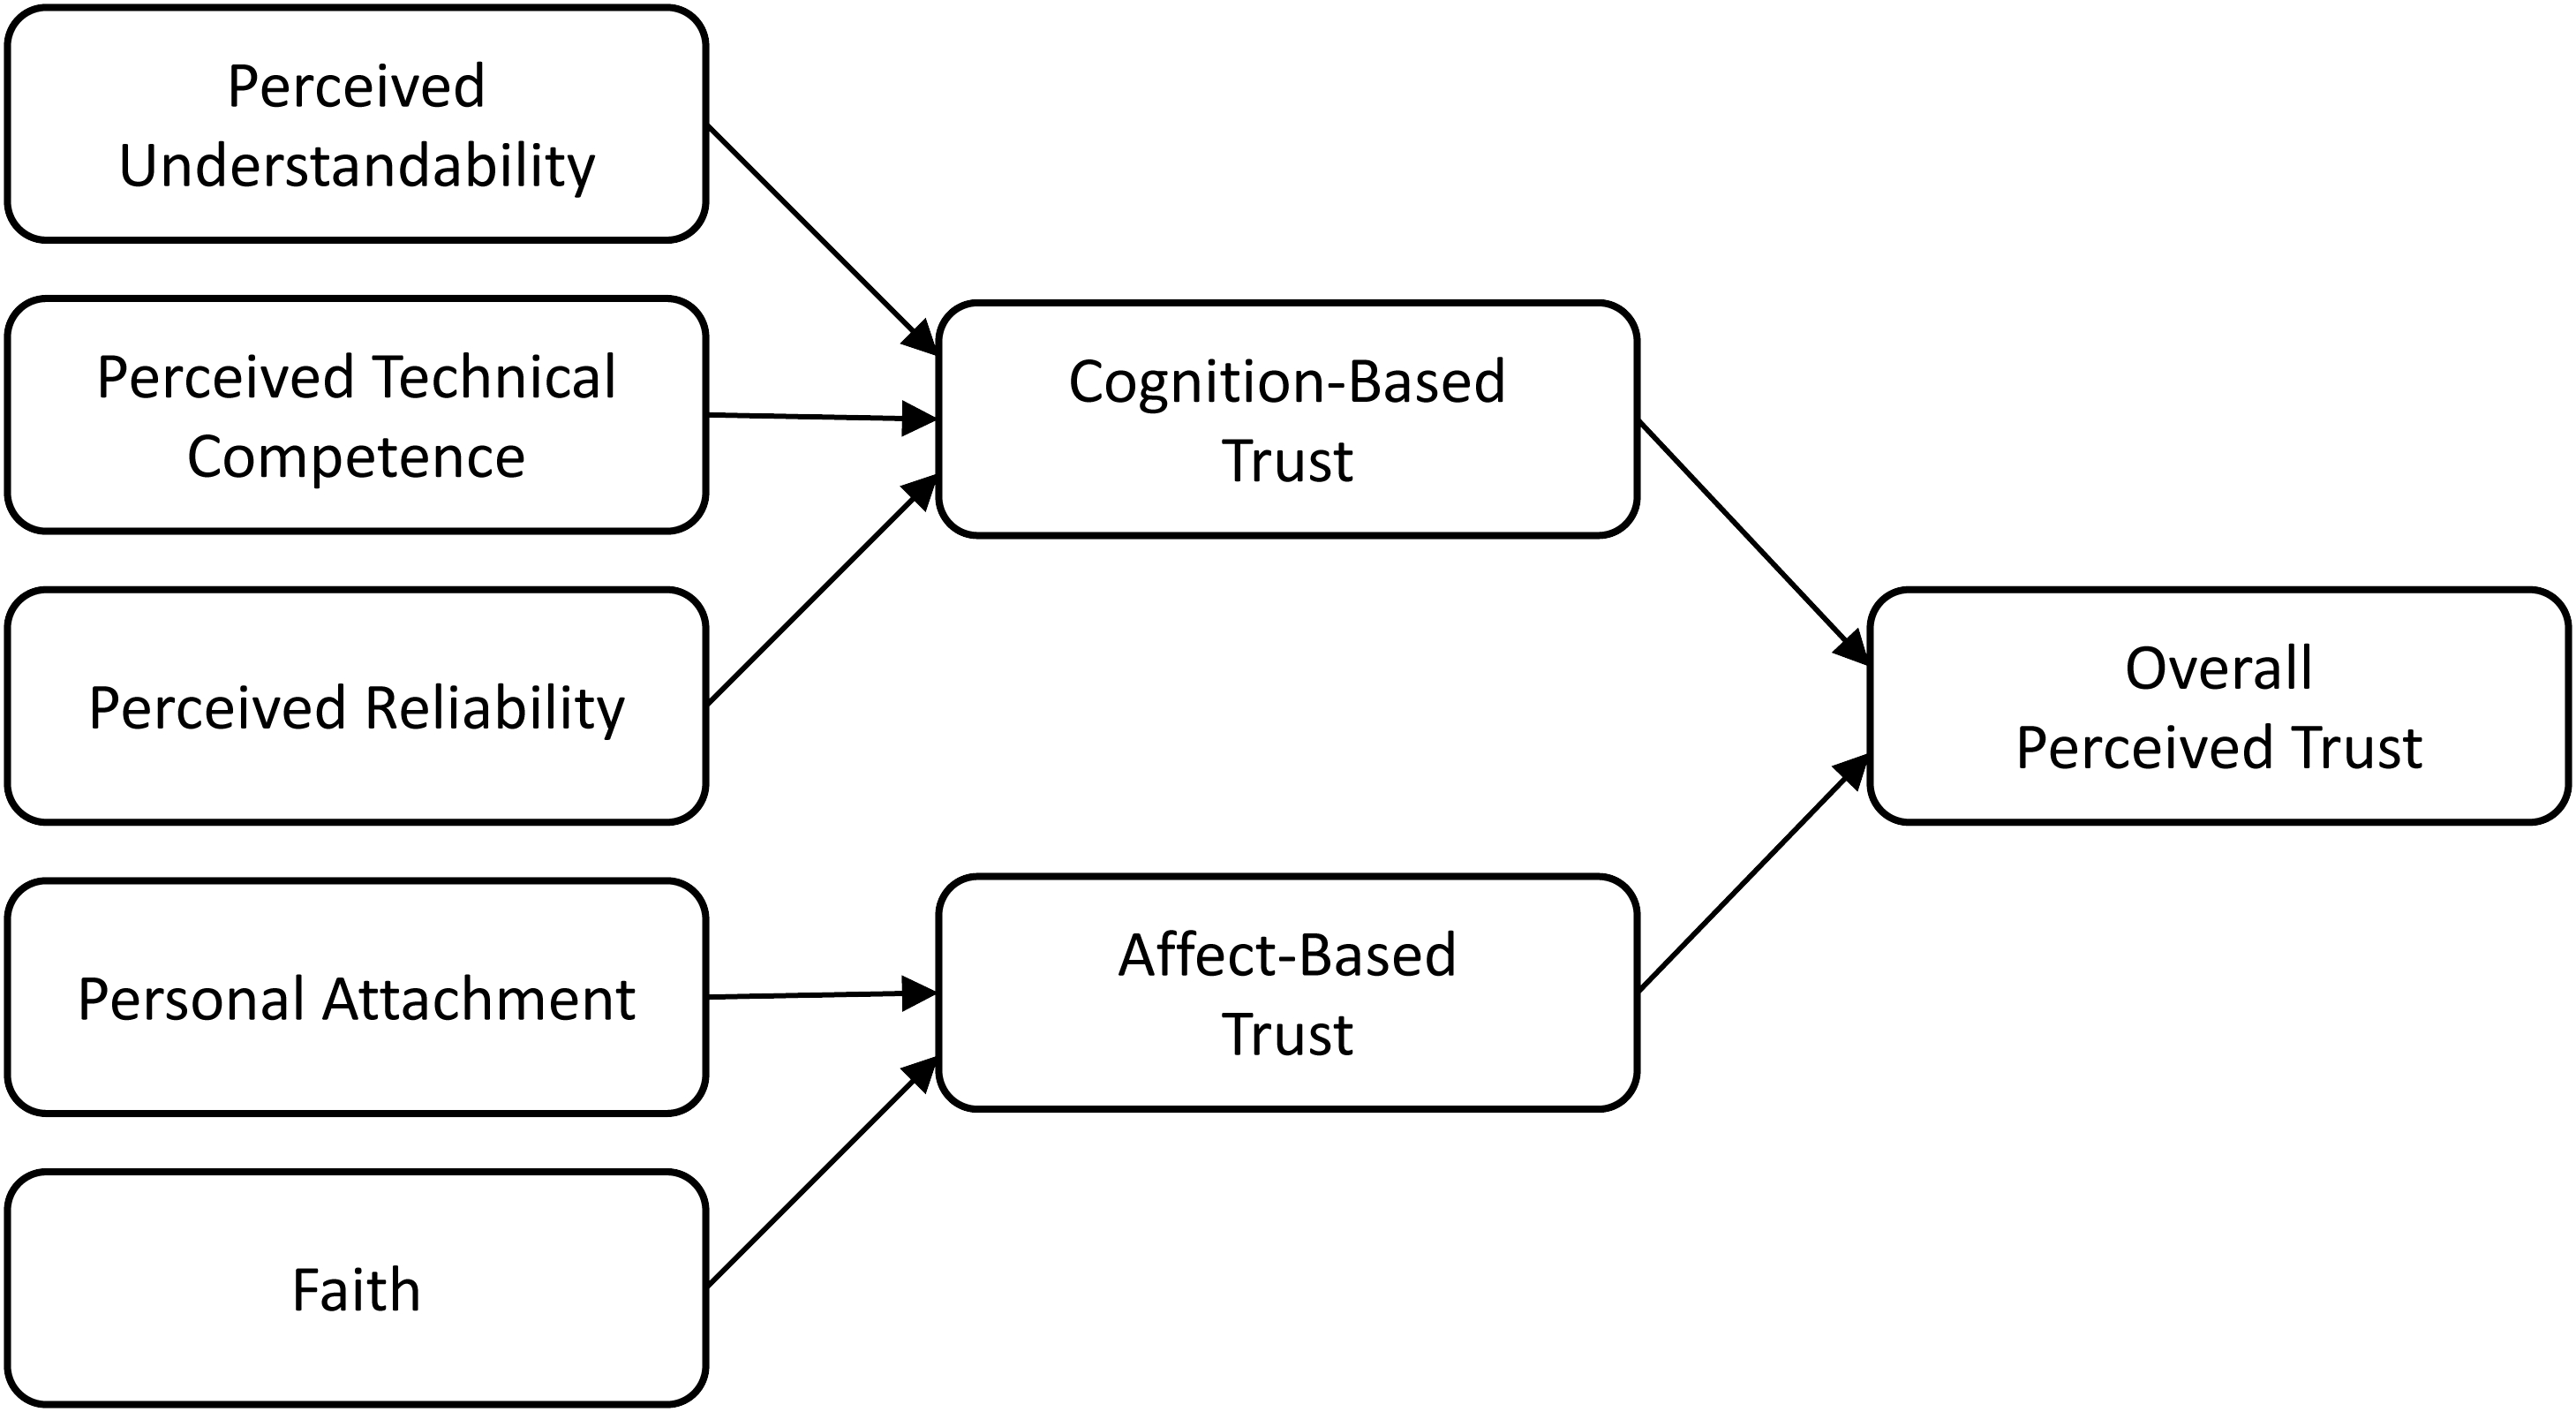
\includegraphics[width=12cm]{trust.png}
	\caption{This is the human-system trust model upon which the original paper founds its explanations.}
	\label{fig:hs_trust}
\end{figure}

For a human-system trust relationship, trust can be separated into nine basic constructs as seen in Figure \ref{fig:hs_trust}. Note that four constructs are left out due to representative and discriminative issues. The five concepts were chosen in the source because they represent a good 68.9\% of the variance in the data set of trust concepts that are important to the overall perceived level of trust based on a PCA\footnote{PCA stands for "Principal Component Analysis" and is a mathematical procedure for transforming a set of possibly correlated values into a smaller set of uncorrelated values.} \cite{htc}.

This gives us five basic constructs of trust with which to work off of. However, only the cognition-based trust concepts can be directly controlled with explanations, as affect-based trust concepts lie beyond the capabilities of the system to influence by explanations. Affect-based trust must be controlled by different means. Concerning the overall perceived level of trust, all five constructs must be perceived to be high. If just a single concept of trust is low, the overall trustworthiness suffers \cite{htc}. Given that we require working knowledge of the level of trust, we need to know the levels of trust that the trustor is perceiving. This proves to be difficult though because they can only be measured with a questionnaire, which is not something a companion system can do whenever trust must be measured – yet.

To enable a companion system to at least have a broad grasp of the measure of trust, the original paper employs reinforcement learning. With it, the system tries to find a solid trade-off between the exploitation of knowledge and the exploration of new aspects. Reinforcement learning is an area of machine learning that tries to teach a system to take actions based on the goal of a perceived reward. Here, the goal likely is a higher level of trust as recognized by the companion system.

In the original paper, these decisions are made based on handcrafted policies, as a statistical approach is not viable due to a lack of data and a lack of method to get this data. In the future, these handcrafted policies can probably be replaced by data collected from a multitude of users, possibly in a non-static way so that the data is always kept accurate. Making an AI or companion system aware of the level of trust between itself and a user still poses a problem and can be an area of further research.

\section{Countering Trust Issues}

Given that we now have a measure of trust, the next step in solving a trust issue is how to counter it. In the original paper, this is done solely by applying explanations to a situation. Alternatively, one could also try to influence the affect-based trust issues.

Simply explaining everything is not the way to correctly implement countering trust issues, however – too many explanations make the usage of a companion system more a hurdle than a plus, as they could lengthen the solving of a problem with unneeded dialogue. This means that we need to know two things: what problems a user will normally face while using a companion system and which events should trigger an explanation.

We also have to match the different types of trust concepts to the explanations, so that the positive effect can be maximized when giving an explanation. This should be done so that we do not spend too much time on explaining simple things to counter a single trust issue when one explanation can be used to counter many trust issues at the same time.

\section{Explanations}

To understand what the original paper is trying to do, it is necessary to know how explanations are viewed. The definition used is based off of Douglas Walton: a successful explanation is a transfer of understanding between a dialogue system in which a questioner and a respondent take part \cite{walton2004new}.

To fully understand how the original paper goes about implementing explanations in its example for a companion system, two things must be known: on which basis to select what type of explanation and where to set triggers to use an explanation in a dialogue.

\subsection{Selecting Explanations}

When selecting an explanation, one must consider the goal of the explanation. There are five goals that the original paper lists. Figure \ref{fig:goals} shows an overview of them.

\begin{figure}[H]
	\centering
	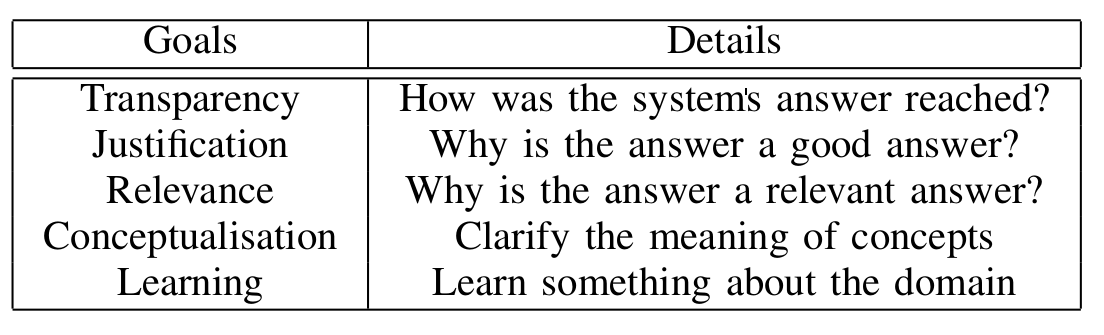
\includegraphics[width=10cm]{goals.png}
	\caption{The goals of explanation.}
	\label{fig:goals}
\end{figure}

The following exposition of the explanations all use the example from the original paper. That is a companion system that helps the user connect a television device to peripheral devices such as a Blu ray player or television tuner. Also, for sake of simplicity we have opted for active examples; examples where the system responds to a user input and not an internal stimulus such as the knowledge graph mentioned later in Section \ref{know_graph}.

\paragraph{Transparency.} The first goal for explanations is transparency. This type of explanation helps the user understand how the companion system reached a given answer and can be used to counteract the low perceived understandability of the system. A user would likely want such an explanation whenever the thought process is not apparent, either because the answer deviates from the expected outcome or when the answer is important enough to warrant that the user needs to know all the factors the system used in reaching the answer. An example of a question that needs this type of explanation is when the user asks: "How did you come to that conclusion?". To that the companion system can then transparently lay out the facts that lead it through its reasoning process.

\paragraph{Justification.} Next is the goal of justification. Here, the user wants to be assured that the companions system has given a good, practical answer, and not just any one that would do. This explanation can be used to counter lack in perceived technical competence and perceived reliability. The system should give such an explanation when it is important for the user to understand that the system gave the best answer to a situation based on its knowledge. An example here would be when a user asks: "Why use a HDMI\footnote{HDMI stands for "High-Definition Multimedia Interface" and is a cable interface for transmitting audio and video.} cable for this connection?". Here, the companion can justify itself by explaining the available alternatives and why it chose the one it did.

\paragraph{Relevance.} Relevance is important to reassure the user that the companion system is aware of the context an answer was sought for in and that the answer is related. This goal of explanations can be used to counter a low perceived reliability. An example for this is: "Why is explaining what HDMI is important for the next step?". Now the companion system has to explain why the information is relevant (possibly because it will be required for the next step, in this case).

\paragraph{Conceptualization.} Another goal of explanations is conceptualization. This is used to clarify the meaning of concepts to a user. The goal can be utilized to strengthen the perceived reliability, technical competence, and understandability all at the same time. This goal most closely resembles the transfer of knowledge from the companion system to the user. For example, this type of explanation can be used when a question such as "What is HDMI?" is asked, to which the system can then provide an answer.

\paragraph{Teaching.} The last goal of explanations is teaching. Here, the companion system aims to teach the user something on the domain of a problem or the domain of a given answer. This goal of explanation can be used to enrich the perceived understandability, as a broader user knowledge allows the system to appear more competent to her. In the given example this could be a fitting explanation to a question like: "What is a male port of a HDMI cable?" to which the companion system can teach the user the difference between the types of ports and how they look like for a HDMI cable.

As one can see, types of explanation can follow one or more goals of explanation – meaning we can counter multiple trust issues with a single explanation if we so wish. This can also be used to only target specific goals when so desired.

On a technical note on selecting explanations, the original paper looks into the architecture of a companion system. Utilizing an explanation machine to select an explanation, the system has to cope with a few uncertainties. Based on the different concepts of trust as seen in Figure \ref{fig:hs_trust}, the companion can select which type of explanation it needs to raise the level of trust between it and the user. Of course, when generating the explanations within the companion system, the explanation also needs to fit into the flow of the current dialogue – this can also be used to refine the selection of explanations.

\subsection{Where to Use Explanations}
\label{know_graph}

Apart from selecting the correct explanation, it is also important to know when to give an explanation. To do this successfully, the original paper uses a large knowledge base upon which the companion system can base its decisions. We also need to know an approximation of how much the user knows – this is done with a user based knowledge graph which represents the knowledge the user has. By comparing the two, the companion system can then decide when and where explanations can be required.

A knowledge graph or base is a specific way of interlinking information in a database, so that associations and connections can be utilized by the computer working off it. In it, the vertices represent chunks of information. The edges connect different vertices through semantic links and associations within the information chunks. In this context, the companion system can start at any vertex and find similar and relevant further information by simply traversing the edges to surrounding vertices.

These knowledge graphs the original paper utilizes are of significant importance to how the companion system handles explanations, so let us take a better look at them. The knowledge base consists of the user profile, environmental information, and the dialog history. When in a dialog, the system can, based on the information saved in the knowledge graph, notice when the knowledge of the user is not sufficient enough for a situation. This can be used to trigger an explanation to impart knowledge on the user, allowing the knowledge graph of the user to fill the holes, so to speak.

However, the knowledge base of the user is not a static construct, unlike the knowledge graph of the companion system (apart from the fact that the companion system can simply update its knowledge at any time). The reason for this is in that we forget things and that knowledge can fade over time. This brings a degree of uncertainty into the comparison between the two knowledge graphs.

To counter this, the original paper simply has the knowledge graph decay over time. This leads towards a situation where information that is seldom used will be explained more often, as the companion system will know that the user will most likely not remember it. Information that is used more often however will only be repeated the first few times to cement it in the user's knowledge, allowing the companion system at some point in time to pass by the explanation as the user has successfully learned this information and can now utilize it herself.

An example for this decay of knowledge is given in the original paper. If an explanation about the cable type HDMI was given a few minutes ago, the companion system will reduce the explanation a further time around because it reasons that the explanation is still present in the user's knowledge; the user's knowledge graph has not yet decayed the new learned information. However, if the explanation is to be given again a few days later, the system will notice that the information has decayed and will counter that by given the full explanation again.

\section{Architecture}

How would the software architecture for such an explanation capable companion system look like? The original paper proposes a modular approach as seen in Figure \ref{fig:architecture} for a variety of reasons.

\begin{figure}[H]
	\centering
	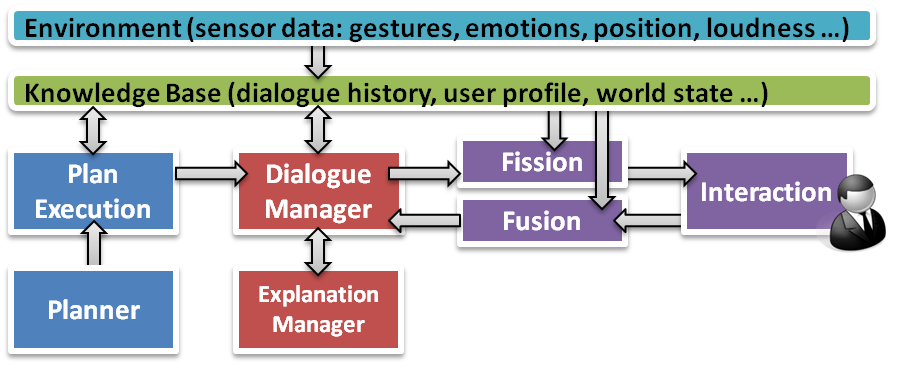
\includegraphics[width=12cm]{arch.png}
	\caption{Overview of the proposed modular architecture for the companion architecture.}
	\label{fig:architecture}
\end{figure}

A few important points lead to the decision for a modular architecture. For one, the use of a platform independent middle-ware for the communication layer between the modules allows for a greater flexibility in how the companion system works and where the modules run, which can be used to separate different parts of the companion system onto different platforms. This platform independent middle-ware also secures trouble-free communication between the modules, even when they are on different platforms using different programming languages or running on different operating system. The original paper utilized the SEMAINE API for this \cite{schroder2010semaine}.

\begin{figure}[H]
	\centering
	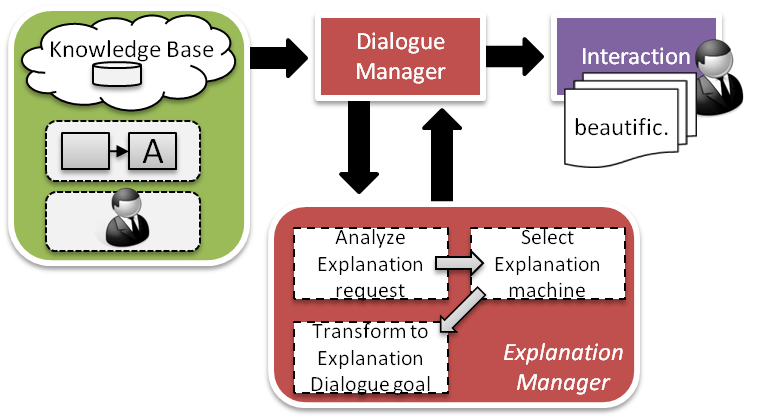
\includegraphics[width=12cm]{expl_arch.png}
	\caption{Close look at the proposed explanation architecture. The dialogue manager processes the explanation requests which are forwarded to the explanation manager. All required information comes from the knowledge base.}
	\label{fig:expl_architecture}
\end{figure}

As can be seen in Figure \ref{fig:expl_architecture}, the explanation manager directly ties in with the dialogue manager. This is because explanations have little impact in how the companion system plans a task or with which media the dialogue is being conducted (these things are tasks of other modules, which in turn do not need to interface with the explanation manager in any way). Therefore, a connection to either the planning modules or the fission and fusion modules is not needed. {\it Fusion} describes the collection of all available input channels into a single, machine understandable one; {\it fission} expands the simple machine output channel into any multitude of output channels available. The explanation machine itself is completely modality independent, meaning that it can be used without outside reliances.

Therefore, the dialogue manager is in charge of deciding when an explanation is required. The explanation manager then analyzes the explanation request based on how the user goals map to the explanation goals and, of course, on what content the user needs to have explained. Then it selects an appropriate explanation machine, which is then transformed to an explanation dialogue goal. All information that is required in these steps comes from the knowledge base of the companion system. The finished explanation is then passed back to the dialogue manager which integrates it into the dialogue with the user.

Apart from the explanation manager, the planner and the dialogue manager are also important parts of the architecture of the proposed modular setup for a companion system. The complete steps from plan to execution can be seen in Figure \ref{fig:planner} – note that the explanation manager is not shown as it is an extra feature not strictly required for the process.

\begin{figure}[H]
	\centering
	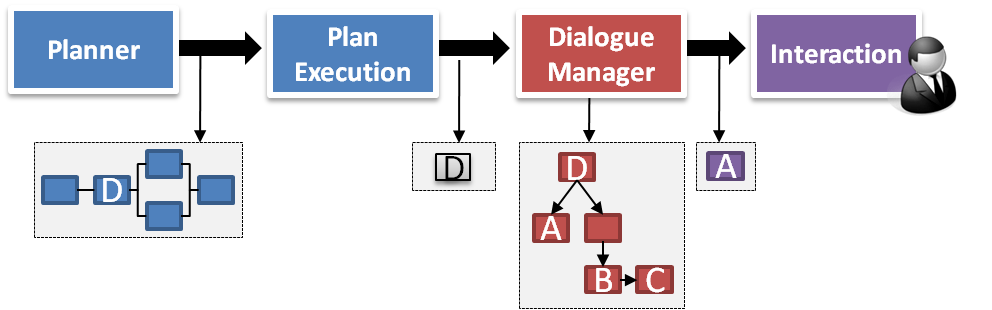
\includegraphics[width=12cm]{planner.png}
	\caption{The path from plan to dialogue.}
	\label{fig:planner}
\end{figure}

The {\it planner} is the module that, given a problem to solve, has to create a plan to solve the given problem – not an easy task, although research has been ongoing as to be seen in \cite{seegebarth2011formale}. Such research has the goal of allowing algorithms to be created that can solve problems in a given domain field on par with human experts. To do this, they must, given a starting state, goal state, and actions, find a path from the start to the goal by applying actions, thus merging the start state into the goal state. This research is generally a part of all planning systems, of which companion systems share aspects of.

The {\it dialogue manager} receives only the abstract steps of the plan from the before mentioned planner and creates a dialogue from it so that the user can solve the given problem. This abstract plan is not enough to create the dialogue, however. The dialogue has to instruct the user on how to solve the task in a way that is adapted and tailored to the user. Therefore, the dialogue manager should also closely interact with the explanation manager, of course, and should the plan need to be amended, it will need to interact with the planner again. Note that this means that the dialogue is not static; it can be changed during run-time to accommodate new circumstances, thus allowing the companion system to adapt as required in Section \ref{adaptive_companion}.

Finally, for actually making the companion system capable of holding a natural dialogue with the user, fusion and fission modules are required. Not only do they abstract the input and output mechanisms for the rest of the system, they are also used to interpret and create natural speech for the communication with the user. Such beautification is done by a {\it natural language pipeline}, as seen in \cite{reiter2000building}, which has the goal of creating fluid human comprehensible text out of the abstract representations the system uses.

\section{Conclusion}

The conclusion of the original paper is that explanations are a viable way to counter trust issues and that companion systems should contain explanation capabilities. It is also pointed out that companion systems can benefit from multimodal input from different sources, given by the fusion module. They also state that it is apparent that there can not be just a single pipeline for explanations, as the events triggering explanations vary in their demands and their contents. Further research must be done, especially on the handling of trust issues so that the explanation pipeline can be further refined. The connection between bases of trust and explanation machines must also be verified in further experiments, hopefully leading to well-founded selection strategies when choosing an explanation.

The original paper also defends its use of a modular architecture, stating that it has definite beneficial sides for an adaptive companion system, as the modular approach allows an easier implementation of the adaptive dialogue structure required.

In the future, a companion system as has been shown in this paper will certainly become more and more sophisticated. Once research has been made into how such a system could reliably measure the trust between the user and itself, the system will only become better and better at giving explanations at the appropriate times within a natural dialogue with a user. As could be seen, constructing explanations is not the main difficulty; instead, when to give an explanation when the user has not explicitly asked for one is the challenging part; also what type of explanation to give based on which trust bases remains challenging. The work of the original paper clearly goes towards teaching companion systems how to act on their own, at least in a dialogue with a user.

\newpage
\bibliography{doc}

\end{document}